\documentclass{standalone}
\usepackage{ tikz }
\usepackage{ xparse }
\input{macros/all}

\begin{document}
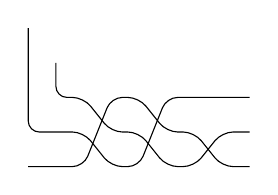
\begin{tikzpicture}[yscale=-1,x=1em,y=1.25em]
        
    \draw [rounded corners] (0,2) -- (2,2) -- (3,0) -- (4,0) -- (5,1) -- (6,1) -- (7,2) -- (8,2);
    \draw [rounded corners] (1,-1) -- (1,0) -- (2,0) -- (3,1) -- (4,1) -- (5,2) -- (6,2) -- (7,1) -- (8,1);
    \draw [rounded corners] (0,-2) -- (0,1) -- (2,1) -- (3,2) -- (4,2) -- (5,0) -- (7,0) -- (8,0);

\end{tikzpicture}
\end{document}